\documentclass[10pt, a4paper]{article}
\usepackage[utf8]{inputenc}
\usepackage{amsmath}
\usepackage{amssymb}
\usepackage{graphicx}
\usepackage{enumitem} % For custom list formatting
\usepackage{tikz} % For drawing simple diagrams
\usepackage{geometry} % To manage page margins
\usepackage{fancyhdr} % For header/footer control

% Set margins aggressively to maximize space and ensure 2-page fit
\geometry{
    a4paper,
    total={190mm,277mm},
    left=13mm,
    right=13mm,
    top=12mm,
    bottom=12mm,
}

\pagestyle{empty}

% Line commands that DO NOT overflow
\newcommand{\writingline}{\rule{0.95\linewidth}{0.4pt}}
\newcommand{\shortline}{\rule{0.3\linewidth}{0.4pt}}

\begin{document}
\begin{center}
    {\small \textbf{IA Competitive Programming Club}} \\
    {\Large\textbf{Introduction to Graphs Worksheet}} \\
    {\small December 09, 2025}
\end{center}

\vspace{0.3cm}
\textbf{Name:} \rule{0.45\textwidth}{0.4pt} \quad \textbf{Date:} \rule{0.3\textwidth}{0.4pt}

\vspace{0.4cm}
\begin{enumerate}[label=\textbf{\arabic*.}]
    
    \item \textbf{Core Terminology (Fill-in-the-Blank)}
    \vspace{0.1cm}
    \begin{enumerate}[label=(\alph*)]
        \item A graph where all edges have a numerical value associated with them is called a \rule{0.2\linewidth}{0.4pt} graph.
        \vspace{0.3cm}
        \item The most space-efficient representation for a \textbf{sparse} graph in competitive programming is the \newline  \rule{0.4\linewidth}{0.05pt}.
        \vspace{0.3cm}
        \item The number of edges connected to a specific vertex is called its \rule{0.2\linewidth}{0.2pt}.
        \vspace{0.2cm}
        \item A graph that contains a path that starts and ends at the same vertex is called \rule{0.3\linewidth}{0.4pt}.
        \vspace{0.3cm}
        \item A tree is a special type of graph that is undirected, connected, and \rule{0.3\linewidth}{0.4pt} (meaning it has no cycles).
    \end{enumerate}

    \vspace{0.4cm}
    \item \textbf{Graph Representation Efficiency}
    
    You are designing a solution for a problem where the graph has $V=10^5$ vertices and $E=10^6$ edges.
    \vspace{0.2cm}
    \begin{enumerate}[label=(\alph*)]
        \item What is the approximate space complexity (in terms of $V$ and $E$) for an Adjacency Matrix representation? \shortline
        \vspace{0.3cm}
        \item Calculate the approximate memory space required for the Adjacency Matrix (assuming one cell stores 4 bytes). \shortline (Approximate total bytes)
        \vspace{0.3cm}
        \item What is the approximate space complexity for an Adjacency List representation? \\\shortline
        \vspace{0.1cm}
        \item Which representation should you choose for this problem, and why? \newline
        \vspace{0.1cm}
        \rule{0.8\linewidth}{0.2pt}.
        \vspace{0.25cm}
    \end{enumerate}

    \vspace{0.4cm}
    \item \textbf{Analyzing a Sample Graph}
    
    Consider the undirected, unweighted graph shown below.
    
    \begin{center}
    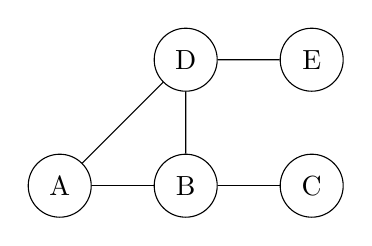
\begin{tikzpicture}[scale=0.8, every node/.style={draw,circle,minimum size=0.8cm,inner sep=0pt}]
        \node (A) at (0, 0) {A};
        \node (B) at (2, 0) {B};
        \node (C) at (4, 0) {C};
        \node (D) at (2, 2) {D};
        \node (E) at (4, 2) {E};
        
        \draw (A) -- (B);
        \draw (B) -- (C);
        \draw (A) -- (D);
        \draw (D) -- (E);
        \draw (B) -- (D);
    \end{tikzpicture}
    \end{center}
    
    \vspace{0.3cm}
    \begin{enumerate}[label=(\alph*)]
        \item What is the degree of vertex B? \shortline
        \vspace{0.2cm}
        \item Write the Adjacency List for the graph above.
        \begin{itemize}[noitemsep, topsep=0pt, parsep=0pt, leftmargin=1.5cm]
            \item A: \rule{0.5\textwidth}{0.4pt}
            \item B: \rule{0.5\textwidth}{0.4pt}
            \item C: \rule{0.5\textwidth}{0.4pt}
            \item D: \rule{0.5\textwidth}{0.4pt}
            \item E: \rule{0.5\textwidth}{0.4pt}
        \end{itemize}
        \vspace{0.2cm}
        \item List one cycle in this graph (e.g., A-B-C-A). \rule{0.3\linewidth}{0.4pt}
    \end{enumerate}

    \newpage

    \item \textbf{Breadth-First Search (BFS) Traversal}

    BFS uses a \textbf{Queue} and finds the shortest path in an unweighted graph. For the graph in Problem 3, simulate the steps of BFS starting from vertex \textbf{A}.

    \vspace{0.2cm}
    \begin{enumerate}[label=(\alph*)]
        \item What is the order in which the vertices are \textbf{visited} (printed/processed)?
        \textbf{Start:} A \quad \rule{0.2\linewidth}{0.4pt}
        \vspace{0.3cm}
        \item What is the shortest distance (in number of edges) from A to C? \shortline
        \vspace{0.3cm}
        \item What is the key advantage of using BFS for pathfinding in unweighted graphs? 
        \vspace{0.1cm}
        \rule{0.2\linewidth}{0.2pt}
        \vspace{0.25cm}
        \writingline
    \end{enumerate}

    \vspace{0.4cm}
    \item \textbf{Depth-First Search (DFS) Traversal}

    DFS uses \textbf{Recursion} (or a Stack) and explores deeply before backtracking. For the graph in Problem 3, simulate the steps of DFS starting from vertex \textbf{A}. Assume neighbors are visited alphabetically.

    \vspace{0.2cm}
    \begin{enumerate}[label=(\alph*)]
        \item What is the order in which the vertices are \textbf{visited} (printed/processed)?
        \textbf{Start:} A \quad \rule{0.2\linewidth}{0.4pt}
        \vspace{0.3cm}
        \item True or False: If you ran a DFS starting at A, you would eventually visit C. \shortline
        \vspace{0.3cm}
        \item What is a primary use case for DFS that BFS is not optimized for? \newline
        \vspace{0.3cm}
        \rule{0.7\linewidth}{0.7pt}
        \vspace{0.25cm}
    \end{enumerate}

    \vspace{0.4cm}
    \item \textbf{Algorithm Selection Challenge}

    For each scenario, identify the most appropriate graph algorithm (BFS, DFS, or neither) and explain your choice.

    \vspace{0.2cm}
    \begin{enumerate}[label=(\alph*)]

        \item \textbf{Scenario:} Determine if you can reach the final commit from the initial commit in a Git repository (a DAG).
        \begin{itemize}[noitemsep, topsep=0pt, parsep=0pt, leftmargin=1.5cm]
            \item \textbf{Algorithm:} \shortline
            \item \textbf{Reason:} \rule{0.75\linewidth}{0.4pt}
        \end{itemize}
        \vspace{0.3cm}

        \item \textbf{Scenario:} A delivery robot must find the route with the fewest intersections in an unweighted map.
        \begin{itemize}[noitemsep, topsep=0pt, parsep=0pt, leftmargin=1.5cm]
            \item \textbf{Algorithm:} \shortline
            \item \textbf{Reason:} \rule{0.75\linewidth}{0.4pt}
        \end{itemize}
        \vspace{0.3cm}

        \item \textbf{Scenario:} You need the shortest path between two cities when roads have varying distances (weights).
        \begin{itemize}[noitemsep, topsep=0pt, parsep=0pt, leftmargin=1.5cm]
            \item \textbf{Algorithm:} \shortline
            \item \textbf{Reason:} \rule{0.75\linewidth}{0.4pt}
        \end{itemize}

    \end{enumerate}

\end{enumerate}

\end{document}
